\documentclass[11pt]{amsbook}

\usepackage[turkish]{babel}

%\usepackage{../HBSuerDemir}	% ------------------------
\usepackage{../Ceyhun}	% ------------------------
\usepackage{../amsTurkish}
\usepackage{graphicx}
\graphicspath{{image/}}

\begin{document}
% ++++++++++++++++++++++++++++++++++++++
\hPage{ceyhun/168}
% ++++++++++++++++++++++++++++++++++++++

\subsection{t-Kesitleme matrisinin gerçekleştirimi}
    \begin{figure}[h]
    	    \begin{enumerate}[label=(\alph*)]
        	    \item    
                	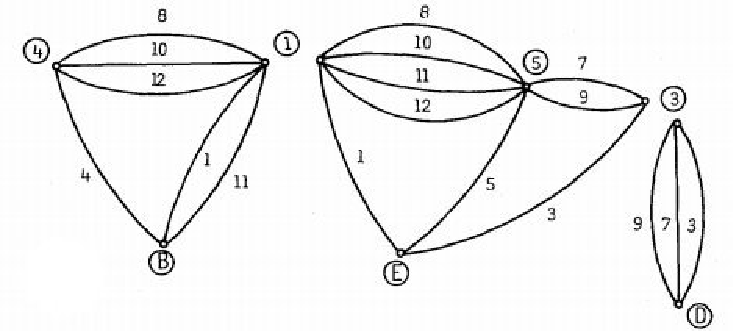
\includegraphics[width=10cm]{images/ceyhun-168-fig01}
            	\item
            	    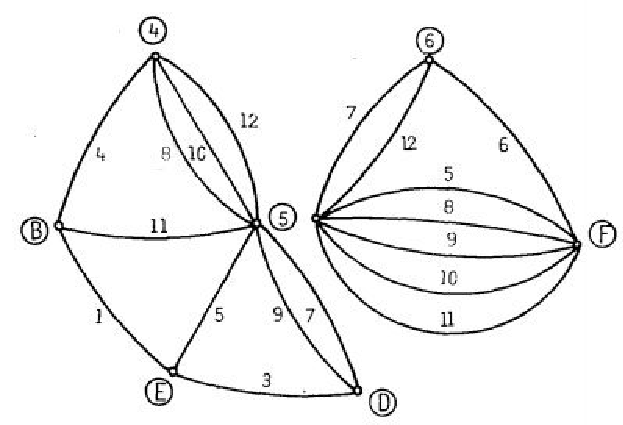
\includegraphics[width=10cm]{images/ceyhun-168-fig02}
        	    \item
            	    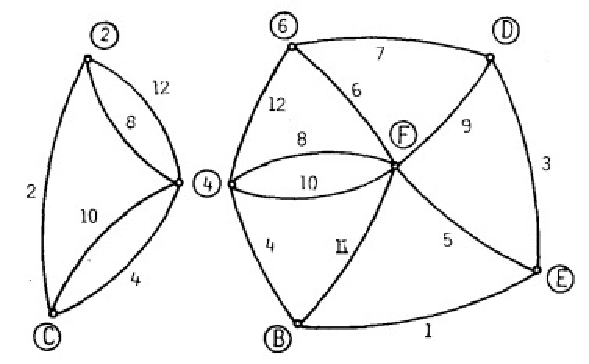
\includegraphics[width=10cm]{images/ceyhun-168-fig03}
            \end{enumerate}
        \label{fig:fig1}
    \end{figure}

\end{document}